\section{Beschreibung der Detektorgeometrie}
Beim einzigartigen QUAD-Detektor (\cref{fig:aufbau_foto} B) von \textit{Bruker Nano} handelt es sich um einen 4-Kanal SDD. Die vier baugleichen, voneinander unabhängigen, nierenförmigen SDD-Zellen sind symmetrisch so um das Pinhole angeordnet, dass sie einer Kreisscheibe möglichst nahe kommen, ohne das Pinhole zu verdecken. Zum Schutz vor Fotoelektronen ist ein \SI{0.5}{\micro\meter} dickes Mylar-Fenster  angebracht. Durch dieses können Elektronen bis maximal etwa \SI{3}{\kilo\electronvolt} abgeschirmt werden. Durch das Pinhole wird der von der Zonenplatte fokussierte Strahl auf die Probe gebracht. Dementsprechend zeigen die Detektorflächen in Strahlrichtung und sitzen möglichst parallel gegenüber zur Probenoberfläche. Der Chip des QUAD-Detektor ist quadratisch und besitzt eine Außenkantenlänge von \SI{14}{\milli\meter} obwohl die Breite der aktive Fläche kleiner ist. Die Gesamtfläche einer nierenförmigen Zelle beträgt \SI{11.2}{\square\milli\meter}. Vom äußersten Rand der Nierenzellen ($r_a=$ \SI{5.1}{\milli\meter}) ausgehend, decken die 4 Zellen gemeinsam 54.8\% der Kreisfläche mit gleichem Radius ab.
\begin{figure}[H]
  \centering
     \includegraphics[width=0.9\textwidth]{illustrations/aufbau-foto_hanna.png}
  \caption[Foto der Optiken und des QUAD-Detektor]{Foto des optischen Aufbaus um den QUAD-Detektor. A) zeigt die Zonenplatte und OSA auf einem röhrenförmigen Support. B) links: QUAD-Detektor in Seitansicht; rechts: in Draufsicht. C) zeigt eine Probe auf der Scanner-Stage, D) Phosphorschirm \cite[S.~41]{hanna}.}
  \label{fig:aufbau_foto}
\end{figure}
Soll der detektierte Raumwinkel maximiert werden, gilt es zu beachten, dass durch den Metallrahmen, welcher den Detektor umgibt Teile der Detektorfläche abgeschirmt werden. Außerdem fügt der Rahmen ein z-Offset $d_{off} = d_{in} + d_{R}$ zum realen Abstand Probenoberfläche zu SDD hinzu. Eine schematische Skizze der Geometrie zwischen Probe und Detektor ist nachfolgend illustriert (\cref{fig:quaddetektor}).
\begin{figure}[H]
  \centering
     \includegraphics[width=0.9\textwidth]{illustrations/winkel.png}
  \caption[Detektorgeometrie im Detail]{Detektorgeometrie im Detail. Im Lot der Probenoberfläche (beige) trifft die Synchrotronstrahlung ein. Davon ausgehend sind die Winkel $\alpha$ und $\beta$ aufgetragen, die den inneren, respektive äußeren Detektionsradius begrenzen. Der Detektor (blau) wird radial durch $r_{max}$ begrenzt. Das Mylar-Fenster (cyan) ist in den Metallrahmen (grau) eingebettet welcher im Abstand $d_{in}$ zum Chip befestigt ist. Der Winkel $\beta$ wird durch eine Kante im Rahmen bei ($r_{Ri},\,d+d_{R}$) begrenzt. Für $\alpha$ müssen die Kanten ($r_{La},\,d+d_{f}$) und ($r_{Li},\,d+d_{L}$) in Betracht gezogen werden. In Millimeter: $r_{Ri}=5.1$, $r_{Li}=2.5$, $r_{La}=1.9$, $r_{max}=7.0$, $d_{in}=0.4$, $d_{R}=1.15$, $d_{L}=0.9$, $d_{f}=0.1$.}
  \label{fig:quaddetektor}
\end{figure}
Zunächst soll berechnet werden für welche Proben-Detektor-Abstände $d$ die Rahmenkante bei ($r_{La},\,d+d_{f}$) und ansonsten die bei ($r_{Li},\,d+d_{L}$) den Innenwinkel $\alpha$ begrenzen. Dazu wird das Koordinatenzentrum in die eintreffende Strahlung auf der Probenoberfläche gelegt. Es lässt sich folgende Steigungsgleichung aufstellen:
\begin{equation}
m = \frac{\Delta y}{\Delta x} = \frac{y_2-y_1}{x_2-x_1} = \frac{(d+d_{L})-(d+d_{f})}{r_{Li}-r_{La}} = \frac{0.9-0.1}{2.5-1.9} = \frac{0.8}{0.6} = \frac{4}{3} .
\end{equation}
Somit ergibt sich der kritische Abstand $d_{crit}$ unter dem die äußere Kante den minimalen Einfallswinkel limitiert zu:
\begin{equation}
d_{crit} + d_f = m \cdot r_{La} \Leftrightarrow (1.9 \cdot \frac{4}{3})-0.1 = d_{crit} = \SI{2.43}{\milli\meter} .
\end{equation}
Das heißt, dass $\alpha$ bei einem Abstand unter $d_{crit} =$ \SI{2.43}{\milli\meter} von ($r_{La},\,d+d_{f}$), überhalb von ($r_{Li},\,d+d_{L}$) begrenzt wird. Daraus ergeben sich folgende Beziehungen für die Winkel $\alpha$ und $\beta$:
\begin{equation} \label{alpha1}
\tan(\alpha) = \frac{r_{La}}{d+d_f} \quad,\quad d \leq \SI{2.43}{\milli\meter}
\end{equation}
\begin{equation} \label{alpha2}
\tan(\alpha) = \frac{r_{Li}}{d+d_L} \quad,\quad d > \SI{2.43}{\milli\meter}
\end{equation}
\begin{equation} \label{beta}
\tan(\beta) = \frac{r_{Ri}}{d+d_R}.
\end{equation}
Im nächsten Schritt soll der detektierte Raumwinkel $\Omega$ bestimmt werden. Der kanonische Raumwinkel (Kreissegment einer Kugeloberfläche) berechnet sich mit dem Öffnungswinkel eines Kegel $\omega$ nach: 
\begin{equation}
\Omega = 2 \pi (1-\cos(\frac{\omega}{2})).
\end{equation}
Der detektierte Raumwinkel ergibt sich also aus der Differenz des doppelten äußeren und inneren Raumwinkels:
\begin{equation} \label{raumwinkel}
\Omega = \Omega_{2\beta}-\Omega_{2\alpha} = 2 \pi (1-\cos(\beta)) - 2 \pi (1-\cos(\alpha)) = 2 \pi (\cos(\alpha) - \cos(\beta)).
\end{equation} % maximize y = 2pi(cos(arctan(2.5/(x+0.9)))-cos(arctan(5.1/(x+1.15))))	% maximize y = 2pi(cos(arctan(1.9/(x+0.1)))-cos(arctan(5.1/(x+1.15))))
Maximieren von \cref{raumwinkel} mit \cref{alpha1} und \cref{beta} liefert ein Maximum $\Omega_{max} = \SI{1.41}{\steradian}$ am Rand bei $d = \SI{2.43}{\milli\meter}$. Die analoge Rechnung mit \cref{alpha2} und \cref{beta} liefert ein lokales Maximum außerhalb des Definitionsbereichs ($<$\SI{2.43}{\milli\meter}).\newlines
Es ergeben sich dadurch im optimalen Probe-Detektor-Abstand ein innerer Öffnungswinkel $\alpha = \SI{36.9}{\degree}$ und ein äußerer Öffnungswinkel $\beta = \SI{54.9}{\degree}$. \newline Das gefundene Ergebnis liegt außerdem innerhalb der Begrenzung der aktiven Zone $r_{max}=\SI{7}{\milli\meter}$: $r = (d+d_R+d_{in})\cdot \tan(\SI{54.9}{\degree}) = \SI{5.64}{\milli\meter}$. \newline
Zudem wird der detektierte Raumwinkel noch durch den nierenförmigen Rahmen gesenkt. Zur Approximation wird die durch die Nieren abgedeckte Fläche im Verhältnis zur Ringscheibe mit gleichen Radien gesetzt, dies entspricht etwa 72\%. Der real detektierte Raumwinkel ergibt sich damit zu $\Omega_{real} = \Omega_{max} \cdot 0.72 = \SI{1.02}{\steradian}$.
\subsection{Absorptionseffekte durch großen Raumwinkel}
Ein großer detektierter Raumwinkel ($>\SI{1}{\steradian}$) ist gleichbedeutend mit einer großen Variation an Beobachtungswinkeln. Dies widerspricht den klassischen Quantifizierungsansätzen für Röntgenfluoreszenzanalyse basierend auf der Sherman-Gleichung, welche mit einer Näherung für kleine detektierte Raumwinkel arbeiten.\newline
Obwohl bereits explizit für große Winkel diverse Ansätze für die Sherman-Gleichung überprüft wurden (Bonizoni et al., 2006; Chang and Wittry, 1994; Malzer and Kanngießer, 2003; Mantler and Kawahara, 2004; Pavlinsky and Kitov, 1979), existiert dafür bisher keine vollständig analytische Integration in die Sherman-Gleichung. Jedoch gibt es für homogene Proben den \textit{equivalent angle}-Ansatz (Malzer und Kanngießer, 2003) welcher zur Quantifizierung dieser Ergebnisse genutzt werden kann. Im Fall von inhomogenen Proben muss jedoch noch ein verlässlicher Quantifizierungsansatz gefunden werden \cite[Abs.~1.2.2]{lars}.